% ================================================================== 14
\section{Anexos}
\label{sec:anexos}

% ------------------------------------------------------------------ A
\subsection{Anexo A. Manual de instalación}
\label{anx:instalacion}

\paragraph{Requisitos.} Python 3.10 o superior y Git. Probado con Python 3.10,
3.12 y 3.13 en Linux y Windows.

\paragraph{Windows con Visual Studio Code.}
\begin{enumerate}
  \item Comprobar Python con \texttt{py --version}. Si no responde, instalar Python
        desde \url{https://www.python.org/downloads/} marcando
        \emph{Add python.exe to PATH}, y reabrir VS Code.
  \item Abrir la carpeta \texttt{ProyectoAlgoritmos} (\emph{Archivo $\rightarrow$
        Abrir carpeta}) y una terminal (\emph{Terminal $\rightarrow$ Nueva terminal}).
  \item Instalar las dependencias y la biblioteca:
\begin{lstlisting}[style=datos]
py -m pip install -r requirements.txt
py -m pip install -e .
py -m rsa_edu --version          # debe responder: rsa_edu 0.2.0
\end{lstlisting}
  \item Si \texttt{gmpy2} no se instala, instalar el resto: es opcional.
  \item La interfaz gráfica usa Tkinter, que viene con el instalador de
        python.org (opción \emph{tcl/tk and IDLE}, marcada por defecto).
\end{enumerate}

\paragraph{Linux o macOS.}\mbox{}
\begin{lstlisting}[style=datos]
git clone https://github.com/kita-02/ProyectoAlgoritmos.git
cd ProyectoAlgoritmos
python3 -m venv .venv && source .venv/bin/activate
pip install -r requirements.txt && pip install -e .
python -m pytest                 # debe terminar con: 397 passed
\end{lstlisting}

% ------------------------------------------------------------------ B
\subsection{Anexo B. Manual de uso}
\label{anx:uso}

En Windows se escribe \texttt{py} en lugar de \texttt{python}.

\paragraph{Interfaz gráfica.} Se abre con \texttt{python -m rsa\_edu interfaz}
(o \texttt{python -m rsa\_edu.interfaz}). Tiene cinco pestañas: \emph{RSA}
(generar claves, cifrar y descifrar de forma directa o con el TCR),
\emph{Exponenciación modular}, \emph{Primalidad}, \emph{Factorización y ataque}
y \emph{Optimización}, que ejecuta el pipeline base y el optimizado con la misma
semilla. Cada pestaña muestra los resultados en tablas con el tiempo y las
operaciones de cada alternativa, y una línea verde ($\checkmark$) o roja ($\times$) que indica si
todas dieron el mismo resultado. La semilla de la parte superior hace que los
datos aleatorios sean reproducibles.

\begin{figure}[H]
\centering
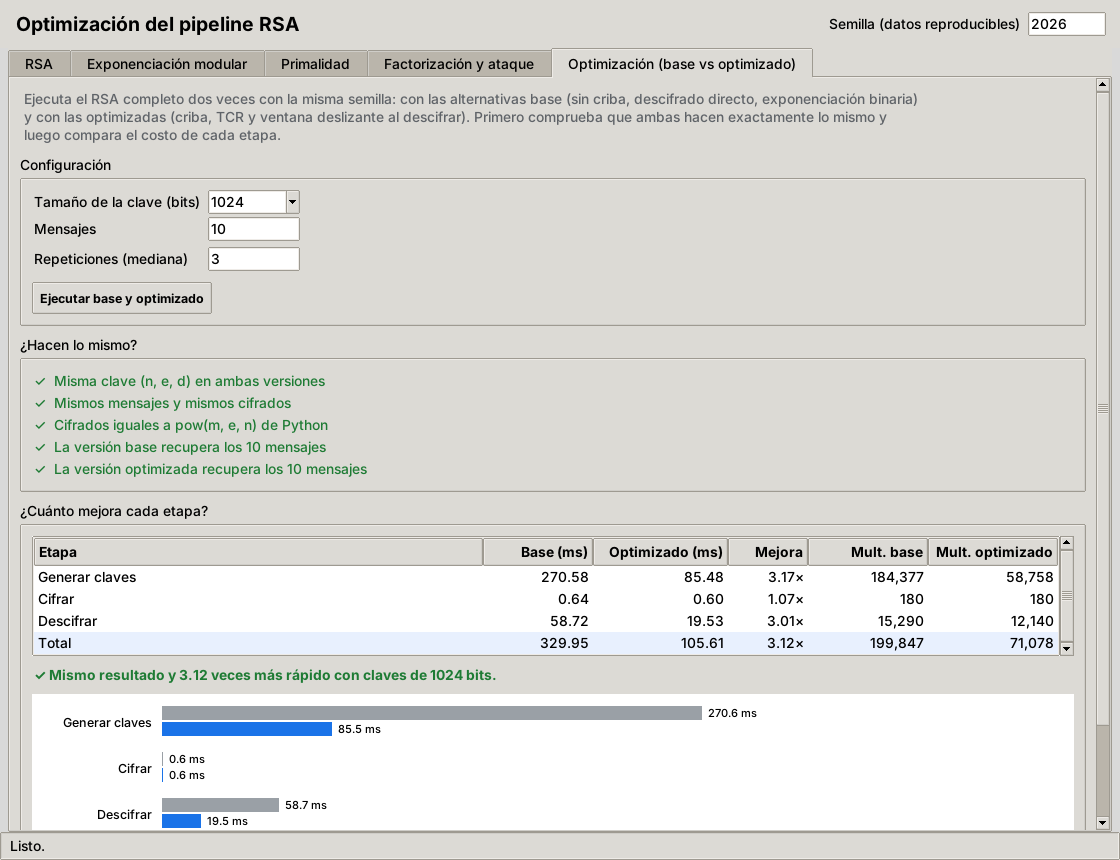
\includegraphics[width=0.9\linewidth]{figuras/interfaz_optimizacion.png}
\caption{Pestaña \emph{Optimización} de la interfaz gráfica (clave de 1024 bits).}
\label{fig:interfaz}
\end{figure}

\paragraph{Línea de comandos.}

\begin{table}[H]
\centering\small
\caption{Subcomandos de la línea de comandos (\texttt{python -m rsa\_edu}).}
\label{tab:cli}
\begin{tabularx}{\linewidth}{@{}>{\ttfamily\footnotesize}R{7.8cm} Y@{}}
\toprule
\textrm{\textbf{Comando}} & \textbf{Qué hace}\\
\midrule
primo 561 [--metodo tentativa | mr | determinista] & Decide si $n$ es primo con el método elegido\\
primo --generar 512 --semilla 7 [--sin-criba] & Genera un primo de 512 bits (con o sin criba)\\
factorizar 3233 --metodo tentativa | rho | brent & Factoriza $n$\\
claves -p 61 -q 53 -e 17 --salida clave.json & Crea la clave del ejemplo manual\\
claves --bits 1024 --salida c.json & Genera una clave según FIPS 186-5\\
cifrar 65 --claves clave.json [--ventana] & Cifra un entero (o \texttt{--texto "..."})\\
descifrar 2790 --claves clave.json [--crt] & Descifra, directo o por TCR\\
atacar -n 3233 -e 17 & Factoriza $n$ y recupera la clave privada\\
comparar primalidad | factorizacion | exponenciacion | descifrado X & Ejecuta todas las alternativas sobre la misma instancia\\
pipeline --bits 1024 [--crt] [--ventana] [--sin-criba] [--gmpy2] & Claves $\rightarrow$ cifrado $\rightarrow$ descifrado con métricas\\
interfaz & Abre la interfaz gráfica\\
\bottomrule
\end{tabularx}
\end{table}

\begin{table}[H]
\centering\small
\caption{Scripts de demostración y de experimentos.}
\begin{tabularx}{\linewidth}{@{}>{\ttfamily\footnotesize}R{7.8cm} Y@{}}
\toprule
\textrm{\textbf{Comando}} & \textbf{Qué hace}\\
\midrule
python scripts/traza\_instancia.py [--p P --q Q --e E --m M] & Traza paso a paso del ejemplo manual, con TCR\\
python scripts/demo\_primalidad.py 61 561 2047 & Compara división, MR y MR determinista\\
python scripts/demo\_factorizacion.py 3233 8051 & Compara división, Rho y Brent\\
python scripts/demo\_optimizacion.py [--bits 2048] & Pipeline base frente a optimizado, mismo resultado\\
python scripts/prototipo\_gmpy2.py & Binaria, ventana, \texttt{pow} y \texttt{gmpy2}\\
python scripts/generar\_instancias.py & Regenera \texttt{data/instancias/} con semilla 2026\\
python scripts/verificar\_reproducibilidad.py & Experimento piloto (dos corridas)\\
python scripts/benchmark.py --config config/preliminar.json & Experimentos preliminares E1--E6\\
python scripts/graficar.py resultados/preliminar & Figuras y tablas\\
python scripts/ajuste\_complejidad.py resultados/preliminar & Teoría frente a mediciones\\
python -m pytest [--cov=rsa\_edu] & Pruebas automatizadas (y cobertura)\\
\bottomrule
\end{tabularx}
\end{table}

\lstinputlisting[style=datos, caption={Flujo completo con la CLI: clave, cifrado, descifrado y ataque.}]{salidas/cli_validos.txt}

% ------------------------------------------------------------------ C
\subsection{Anexo C. Bitácora resumida del grupo}
\label{anx:bitacora}

La bitácora completa está en \texttt{docs/BITACORA\_GRUPAL.md}. Las fechas
corresponden a los commits del repositorio y a las sesiones de avance.

\begin{longtable}{@{}p{1.9cm} p{5.3cm} p{5.0cm} p{2.4cm}@{}}
\caption{Bitácora del grupo: avances, decisiones y cambios.}\label{tab:bitacora}\\
\toprule
\textbf{Fecha} & \textbf{Avance} & \textbf{Decisiones y cambios} & \textbf{Evidencia}\\
\midrule
\endfirsthead
\toprule
\textbf{Fecha} & \textbf{Avance} & \textbf{Decisiones y cambios} & \textbf{Evidencia}\\
\midrule
\endhead
29/09/2026 & Creación del repositorio y estructura inicial de \texttt{rsa\_edu}. & Python con \texttt{int} nativo; código en \texttt{src/}, scripts en \texttt{scripts/}. & commit \texttt{6e6a1d0}\\
06/10/2026 & Prototipo de la Entrega 1: aritmética (Francesco), primalidad (Orlando), factorización (Camila), pipeline RSA básico y traza (Emmi). & Arquitectura en capas; \texttt{\_\_init\_\_.py} no reexporta; un commit por capa e integrante; enteros grandes como texto en JSON. & commits \texttt{e4bec8d}, \texttt{2d35c0b}, \texttt{6a05a21}, \texttt{edcbe25}\\
oct.\ 2026 & Entrega 1: formulación, fundamentos, stack, diseño, ejemplo manual, plan de pruebas y de aprendizaje, prototipo. & Pares de alternativas a comparar; \texttt{gmpy2} solo como opcional (matriz de decisión). & Informe de la Entrega 1\\
23/10/2026 & Segunda alternativa de cada etapa: ventana y \texttt{Contador} (F), MR determinista, criba y \texttt{generar\_primo} (O), Rho con límite, Brent y ataque (C), claves FIPS 186-5, TCR, pipeline, CLI, formatos, benchmark E1--E4 e integración continua (E). & $d$ con $\lambda(n)$ en claves aleatorias; generador aparte para las bases de MR; \texttt{max\_iter}; pila de cofactores; contador opcional; \texttt{generar\_primo} pasa a \texttt{primalidad.py}. & commits \texttt{0f1f299}, \texttt{134881e}, \texttt{9075811}, \texttt{f8b1388}, \texttt{002467a}\\
oct.\ 2026 & Presentación de los avances de implementación (primera y segunda alternativa, integración). & -- & Diapositivas de los avances\\
05/11/2026 & Revisión del repositorio frente a lo presentado. & Se detectan scripts desactualizados en GitHub (traza sin TCR, demo sin Brent, prototipo \texttt{gmpy2} pendiente); se corrigen. & {\footnotesize\texttt{CHANGELOG.md}}\\
06/11/2026 & Diseño experimental E1--E6, piloto, experimentos preliminares, ajuste con la teoría, documentación técnica y demostración de la optimización. & Oráculo \texttt{sympy} en lugar de etiquetas propias; exponentes aleatorios en E3; conteo separado del cronometraje; experimento E6 del pipeline completo; estándares documentados. & commits 1 a 5 y 11 del paquete de la Entrega 2\\
06/11/2026 & Demostración al docente de los algoritmos y de las pruebas automatizadas (tipos de prueba y semillas). & -- & Guía de comandos\\
17/11/2026 & Entrega 2: informe con la estructura final, bitácora grupal y guiones de presentación. & El informe adopta las 14 secciones del informe final. & commits 12 y 13\\
18/11/2026 & Interfaz gráfica pedida por el docente: ventana con cinco pestañas para usar los algoritmos y ver los resultados en tablas y gráficos. & Tkinter (viene con Python); cada integrante programa la pestaña de su módulo; la lógica se separa de la ventana para probarla sin pantalla (pruebas G1--G6). & commits 6 a 10\\
\bottomrule
\end{longtable}

% ------------------------------------------------------------------ D
\subsection{Anexo D. Matriz de contribuciones}
\label{anx:contribuciones}

\begin{table}[H]
\centering\small
\caption{Contribuciones verificables de cada integrante en el repositorio.}
\label{tab:contribuciones}
\begin{tabularx}{\linewidth}{@{}R{2.3cm} Y Y Y@{}}
\toprule
\textbf{Integrante} & \textbf{Código} & \textbf{Pruebas y experimentos} & \textbf{Commits}\\
\midrule
Francesco Canal & \texttt{aritmetica.py} (exponenciación ingenua, binaria y ventana), \texttt{contador.py} & A1--A8, G2; \texttt{prototipo\_gmpy2.py}; \texttt{graficar.py}; pestaña de exponenciación & \texttt{e4bec8d}, \texttt{0f1f299}; paquete E2: 2, 7 y 12\\
Orlando Clemente & \texttt{primalidad.py} (división, MR, MR determinista, criba, \texttt{generar\_primo}) & P1--P11, X1--X6, G3; \texttt{verificar\_reproducibilidad.py}; piloto; pestaña de primalidad & \texttt{2d35c0b}, \texttt{134881e}; paquete E2: 4, 8 y 13\\
Camila Fernández & \texttt{factorizacion.py} (división, Rho, Brent, fachada), \texttt{ataque.py} & F1--F9, G4; \texttt{ajuste\_complejidad.py}; resultados preliminares; pestaña de factorización y ataque & \texttt{6a05a21}, \texttt{faa26b0}, \texttt{9075811}, \texttt{00380c9}, \texttt{dba75ad}; paquete E2: 3, 5 y 9\\
Emmi Huaman & \texttt{rsa.py}, \texttt{pipeline.py}, \texttt{formatos.py}, CLI & R1--R12, I1--I7, G1, G5, G6; \texttt{benchmark.py}; configuraciones; integración continua; ventana principal y pestañas RSA y Optimización & \texttt{6e6a1d0}, \texttt{019623e}, \texttt{edcbe25}, \texttt{f8b1388}, \texttt{002467a}; paquete E2: 1, 6, 10 y 11\\
\bottomrule
\end{tabularx}
\end{table}

\noindent Los commits del «paquete E2» se publican en GitHub al subir la Entrega~2;
cada uno queda a nombre de su autor.

% ------------------------------------------------------------------ E
\subsection{Anexo E. Evidencias de seguimiento}
\label{anx:seguimiento}

\begin{table}[H]
\centering\small
\caption{Hitos de seguimiento y evidencia de cada uno.}
\begin{tabularx}{\linewidth}{@{}R{2.8cm} Y Y@{}}
\toprule
\textbf{Hito} & \textbf{Qué se presentó} & \textbf{Evidencia}\\
\midrule
Entrega 1 & Formulación, diseño, ejemplo manual, plan de pruebas y de aprendizaje, prototipo inicial & Informe de la Entrega 1; commits del 06/10/2026\\
Avances de implementación & Primera y segunda alternativa de cada etapa; integración; demostración con instancias del docente & Commits del 23/10/2026; diapositivas\\
Avances de pruebas y experimentos & Batería de pruebas, análisis de complejidad, diseño experimental, piloto y experimentos preliminares & Commits del 06/11/2026; \texttt{resultados/}\\
Entrega 2 & Este informe; repositorio; interfaz gráfica; demostración & Commits 6 a 13; guiones de presentación\\
\bottomrule
\end{tabularx}
\end{table}

% ------------------------------------------------------------------ F
\subsection{Anexo F. Datos y material complementario}
\label{anx:datos}

\begin{lstlisting}[style=datos, caption={Organización del repositorio (Entrega 2).}]
ProyectoAlgoritmos/
|-- src/rsa_edu/        aritmetica, contador, primalidad, factorizacion, ataque,
|                       rsa, pipeline, formatos, __main__ (CLI)
|     interfaz/         app, comun, componentes y una pestaña por módulo
|-- tests/              15 archivos, 397 pruebas
|-- scripts/            traza, demos, prototipo gmpy2, instancias, benchmark,
|                       verificar_reproducibilidad, graficar, ajuste_complejidad
|-- config/             piloto.json, preliminar.json, experimentos.json
|-- data/instancias/    primos.json, semiprimos.json, adversos.json (semilla 2026)
|-- resultados/
|     piloto/           corrida_1/, corrida_2/, reproducibilidad.md
|     preliminar/       E1.csv ... E6.csv, metadatos.json, figuras/, tablas/, ajustes.md
|-- docs/               DOCUMENTACION_TECNICA.md, BITACORA_GRUPAL.md
|-- informe/entrega2/   este informe (LaTeX y PDF)
|-- .github/workflows/  pruebas.yml (integración continua)
|-- README.md  CHANGELOG.md  requirements.txt  pyproject.toml  pytest.ini
\end{lstlisting}

\lstinputlisting[style=datos, caption={Configuración del pipeline con \texttt{gmpy2}: mismos resultados, otra implementación de la aritmética.}]{salidas/pipeline_gmpy2.txt}

